% Draft #1
\documentclass[12pt,a4]{article}
\usepackage{a4wide}
\usepackage{hyperref}
\usepackage{graphicx}
\usepackage{epstopdf}

\parindent 0pt
\parskip 6pt

\begin{document}
    \thispagestyle{empty}

    \rightline{\large Biko Agozino}
    \medskip
    \rightline{\large St John's}
    \medskip
    \rightline{\large ba325}

    \vfil

    \centerline{\large Part II Project Proposal}
    \vspace{0.4in}
    \centerline{\Large\bf Inferring sequence specifications from drum rhythms}
    \centerline{\large October 22, 2015}

    \vfil

    {\bf Project Originator:} Dr. Alan Blackwell \& Dr. Sam Aaron

    \vspace{0.1in}

    {\bf Resources Required:} Yes, please see \hyperref[sec:Resources]{Resources Required section}

    \vspace{0.5in}

    {\bf Project Supervisor:} Isak Herman

    \vspace{0.2in}

    {\bf Signature:}

    \vspace{0.5in}

    {\bf Director of Studies:} Dr Robert Mullins

    \vspace{0.2in}

    {\bf Signature:}

    \vspace{0.5in}

    {\bf Overseers:} Professor Ross Anderson \& Professor Jean Bacon

    \vspace{0.2in}

    {\bf Signatures:}


    \vfil

    \eject

    \section{Introduction and Description of Work}

Drummers in many contemporary western musical ensembles play a vital role in the performance. They provide the rhythm, tempo, and pace of a song leading to the whole performance depending on the consistency of the drummer. However, Each drummer has their own nuances to their performance that manifest in the form of a slower/faster tempo or softer/harder beats. This can make it difficult to untrained musicians when attempting to reproduce the performance either on a physical drumkit or electronically without sampling. This is because the intended patterns performed by the drummer - of which their own personal transformations have affected - may not be immediately clear.

This project proposes to implement a system that infers the intended sequence of strokes on a drumkit from those that are captured, regardless of the variations in timing of the sequence and missed or incorrect beats. The system will then output the recording as the drum tablature or a MIDI\footnotemark \footnotetext{Musical Instrument Digital Interface} file for the user to either follow for their next performance or for use in their preferred music editing software.

The system will take on several steps, these are described briefly here and detailed further in the \hyperref[sec:ProjectStructure]{Project Structure section}. The system will take in a MIDI input from an electronic drum kit and process it into a timestamped array, this will either be analysed directly or transformed into Drum Tablature before analysis.

Drum Tablature is a simplified form of Drum notation which is popular amongst drummers for its simplicity and ease of access, the contrast between Drum Tablature and standard notation can be seen in Figure \ref{exampleDrumTab}. Drum Tablature is significant as it will be the form of information that we will harvest from a free online database\footnotemark \footnotetext{This database lives on http://drumbum.com/drumtabs/} for use as a training set. This training set will then be used as the prior expectation when inferring the beat that the input is intending to play.

\begin{figure}[h]    
            \centerline{\includegraphics[scale=0.5]{figures/exampledrumtab.eps}\\
            \includegraphics[scale=0.3]{figures/Characteristic_rock_drum_pattern.png}}
    \caption{\label{exampleDrumTab} An example of Drum Tablature vs the standard notation (credit to Wikipedia user:Hyancinth for creating the standard notation). The x axis is essentially time and the y axis is the instrument being used. Varying symbols are used to represent different types of strike}
\end{figure}







    \section{Starting point}
I have experience creating web applications with a Java backend, this will be useful as the main component of the project is planned to be implemented in Java. I have also completed Java practical classes as part of Part IA and Part IB.

The Artificial Intelligence I and Mathematical Methods for Computer Science courses in Part 1B will be useful for the Machine Learning component of this project, particularly the Probability components of the Maths course. Other courses that are likely to provide key assistance are the Information Theory, Natural Language Processing, Digital Signal Processing, and Artificial Intelligence II courses in Part II.


    \section{\label{sec:ProjectStructure}Project structure}

\begin{figure}[h]
    \centerline{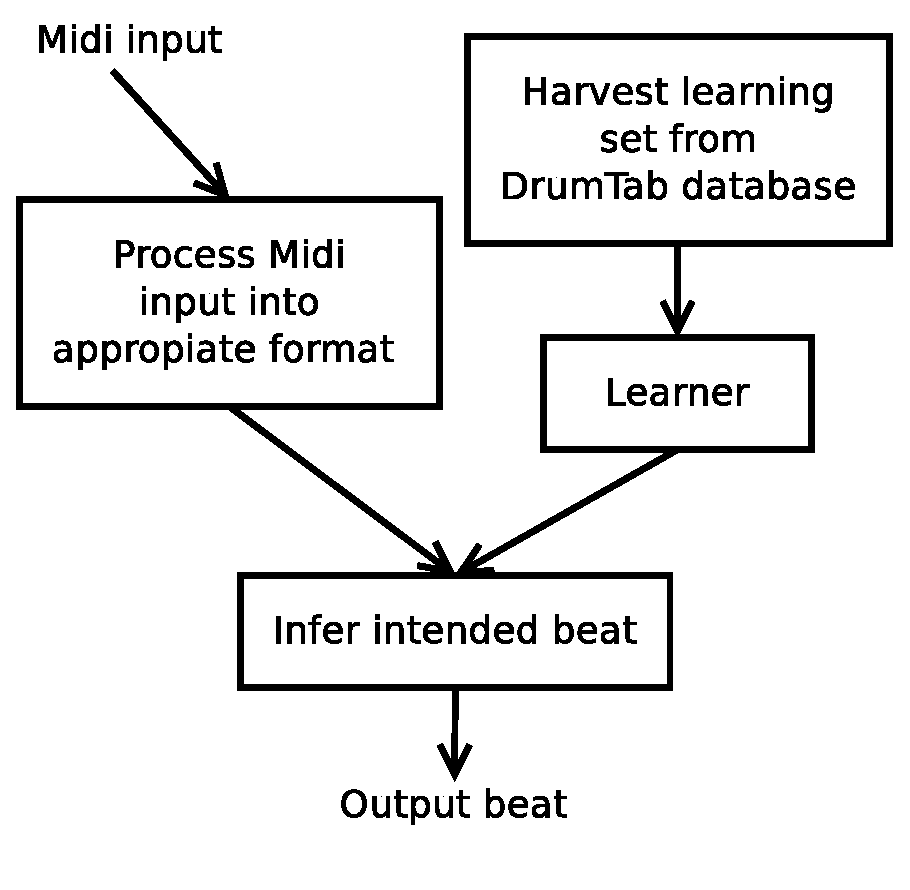
\includegraphics[scale=0.5]{figures/System.eps}}
    \caption{\label{System} The core system}
\end{figure}

To allow for modular design of the system (Figure \ref{System}) the project has been split into the following steps/modules:
        \begin{enumerate}
            \item Read MIDI input data from an electronic drum kit into a time-stamped array. This step represents how the user will input into the system for later analysis by the inference model. It also allows me to get to grips with MIDI programming and prepares me for the steps to come.
            \item Translate the contents of the time-stamped array into Drum Tablature format for comparison with the learning set.
            \item Build the Learning set using a free Drum Tablature database, the learning set will be formed by parsing Drum Tablature into a sequence of beats.
            \item Train a Hidden Markov Model (or other machine learning model if it appears more appropriate at the time) by using the sequences of beats from step 3
            \item Create the inference module by using the trained model as a prior expectation in order to infer the intended sequence from the input of stage 1
        \end{enumerate}

        \subsection{Possible extensions}
The primary extension and stretch goal is to integrate this inference model with the Sonic Pi live coding environment. Live coding is an emerging performing art in which the musician dynamically "codes" music. Integrating this inferred drum pattern into Sonic Pi will be a proof of application for this inference system. It could allow for further extensions in the realms of live programming and using this system as a tool for live performance. One idea is to infer what sequence of beats is likely to follow the one originally played, leading to an automatically developing baseline upon which the performer is free to worry about other details without the piece sounding monorhythmic. This opens the project to the realms of Algorithmic Composition which has been attempted many times, as detailed in this survey\cite{algorithmicCompositionSurvey}.

A further extension is to use an OMR\footnotemark \footnotetext{Optical Music Recognition} system to extend the learning set by parsing the standard drum notation (see Figure \ref{exampleDrumTab}. OMR is a progressing field and this extension could be considered its own project, infact Yipeng Cheng\cite{yipeng} attempted to do just that in 2014. As such it is unlikely for this extension to be implemented, though is an area that may help with any limitations found from using Drum Tablature.

Similarly, the final extension I will detail here is using the Real-time Beat Tracking System, such as the one described by Masataka Goto\cite{Goto01}, to both expand the learning set from audio signals as well as allowing users to input audio into the system for processing and beat inference.
 

    \section{Success Criteria}
The following components are required for the successful development of the project:
        \begin{enumerate}
            \item Implementation of a system that reads MIDI and is able to translate it into Drum Tablature
            \item Implementation of a system that is able to take sets of Drum Tablature as a training set for a Machine Learning model
            \item Implementation of a system that is able to infer the intended drum pattern from an input pattern
            \item Evaluation of whether this inference is correct through one or both of:
                \begin{itemize}
                    \item A human study, where users determine whether the inferred pattern is correct or not
                    \item A statistical study based on whether the inference model is reliable or not
                \end{itemize}
        \end{enumerate}
        \subsection{Evaluation}
Evaluation will take place when the core aims of the project have been completed. This subsection gives more detail to the final success criterion.
\begin{itemize}
    \item{\bf Human Study:} I propose that the human study will take place with a selection of moderately to skilled drummers attempting a beat on the MIDI drum kit. The machine will then infer what beat it expects the user to have been intending to play. For the purposes of this study two other sequences will be selected through some random generation upon the original inferred one. All three will be fed back to the user and it is the user's task to pick the one that they intended to play, this should give us a metric of whether the user can reliably select the inferred beat.
    \item{\bf Statistical Study:} This will be regression analysis on an input into the system and whether the inference model is being consistent with its inference, i.e. is the inference model consistent with its selection of beat?
\end{itemize}

    \section{\label{sec:Resources}Resources Required}
    I will require the following devices:
        \begin{itemize}
            \item \emph{My Computer:} This is a Ubuntu machine with an Intel Dual Core i5 processor and 8 GB of RAM. My contingency plans to protect myself against hardware and/or software failure include using the Git version control system, and hosting all vital files on a GitHub repository. This will mean that I can download the project onto another machine or MCS machine if I needed.
            \item \emph{Roland MIDI drum kit:} This will be used for integration testing as well as gathering initial test data and evaluation. The Rainbow Research Group has agreed to allow me to use theirs.
            \item \emph{Alesis USB MIDI controller} Same as above.
        \end{itemize}
        \subsection{Tools}
            I will be using the following tools as part of my project:
            \begin{itemize}
                \item \emph{Java and IntelliJ:} I will use Java to write the program and the IntelliJ IDE as my development environment for which I have my own (student) license.
                \item \emph{JUnit:} JUnit will be the testing framework used to test individual components.
            \end{itemize}
    \section{Timetable and Milestones}
To allow for regular targets, the remaining time until the submission deadline has be split into 2 week work sections.

        \subsection{23/10/15 - 5/11/15}
        \begin{itemize}
            \item Read further about beat tracking and machine learning models (this will continue throughout the project, gathering a Bibliography to use)
            \item Write and test code for reading MIDI data into a timestamped array
            \item Build a framework for project
            \item Read further about Drum Tablature and its relation to MIDI
        \end{itemize}
{\bf Target:} MIDI data can now be input into the system
        \subsection{6/11/15 - 19/11/15}
        \begin{itemize}
            \item Translate MIDI data into Drum Tablature
            \item Reading about how to parse Drum Tablature
        \end{itemize}
{\bf Target:} MIDI data can now be input into the system and translated into drum tablature
        \subsection{20/11/15 - 3/12/15}
        \begin{itemize}
            \item Compile a learning set from a subset of the data on the DrumTab database
            \item Parse the learning set into a standardised format
            \item Prepare the machine learning model
        \end{itemize}
{\bf Target:} Drum Tablature has now be translated into an accepted format ready for the machine learning model
        \subsection{4/12/15 - 17/12/15}
\begin{itemize}
        \item Implement the machine learning model
        \item Draft introduction and preparation chapters of dissertation
        \end{itemize}
{\bf Target:} Machine Learning Model has been created, ready for the learning set. Introduction and preparation chapters of the dissertation have been drafted and submitted to Supervisor and Director of Studies for review.
        \subsection{18/12/15 - 31/12/15}
\emph{Work in these two weeks will be slowed because of Christmas and New Year}
\begin{itemize}
        \item Read about inference algorithms
        \item Draft progress report
\end{itemize}
{\bf Target:} Progress report up until this point drafted
        \subsection{1/1/16 - 14/1/16}
\begin{itemize}
        \item Implement training algorithm for the Machine learning Model
        \item Test training algorithm

\end{itemize}
{\bf Target:} Machine learning model trained
        \subsection{15/1/16 - 28/1/16}
\begin{itemize}
        \item Implement chosen inference algorithm
        \item Test inference algorithm
        \item Progress report final draft
        \item Prepare progress presentation
\end{itemize}
{\bf Target:} Machine now able to infer beat. Core aims complete. Progress report submitted to Overseers.
        \subsection{29/1/16 - 11/2/16}
        \begin{itemize}
            \item Buffer period for any incomplete work
            \item Start Evaluation
        \end{itemize}
        \subsection{12/2/16 - 25/2/16}
        \begin{itemize}
            \item Sonic Pi integration extension
            \item Evaluation
        \end{itemize}
        {\bf Target:} Inferred beat now able to be exported as a Sonic Pi file
        \subsection{26/2/16 - 10/3/16}
        \begin{itemize}
            \item Write Implementation Chapter
            \item Any further improvements
        \end{itemize}
{\bf Target:} Draft of Implementation Chapter
        \subsection{11/3/16 - 24/3/16}
        \begin{itemize}
            \item Write Evaluation and Conclusions chapters
        \end{itemize}
{\bf Target:} Draft of Evaluation and Conclusions chapters
        \subsection{25/3/16 - 7/4/16}
        \begin{itemize}
            \item Update Introduction and preparation chapters where needed
        \end{itemize}
        \subsection{8/4/16 - 21/4/16}
        \begin{itemize}
            \item Final draft of Dissertation ready for review.
        \end{itemize}
{\bf Target:} Final Dissertation ready for review by Supervisor and Director of Studies
        \subsection{22/4/16 - 5/5/16}
        \begin{itemize}
            \item Buffer period to fix any problems around dissertation
        \end{itemize}
        \subsection{6/5/16 - 13/5/16}
            \begin{itemize}
                \item Submit dissertation and source code
            \end{itemize}
        

    \section{Bibliography}
\begin{thebibliography}{9}
    \bibitem{algorithmicCompositionSurvey}
        George Papadopoulod; Geraint Wiggins,
        \emph{AI Methods for Algorithmic Composition: A Survey, a Critical View and Future Prospects},
        University of Edinburgh,
        1999.
    \bibitem{Goto01}
        Masataka Goto,
        \emph{An Audio-based Real-time Beat Tracking System for
    Music With or Without Drum-sounds},
        Journal of New Music Research, 30:2, 159-171,
        2001.
	\bibitem{yipeng}
	Yipeng Cheng,
	\emph{Optical Music Recognition}
	Part II Project, University of Cambridge,
	2014
    

\end{thebibliography}

\end{document}

